\documentclass[12pt]{article}
 
\usepackage[T1]{fontenc}     
\usepackage[utf8]{inputenc}  
\usepackage[magyar]{babel}   
\usepackage{lmodern}
\usepackage{caption}       
\usepackage{makecell}
\usepackage{boldline} 
 
\usepackage{amsmath,amssymb}
\usepackage{tikz, pgfplots}
\usetikzlibrary{positioning}
\usepackage{arydshln}
\usepackage{booktabs}
\usepackage{multirow}
\usepackage{booktabs} 
\usepackage{amsthm}          
\usepackage{graphicx}  
\usepackage{hyperref}  
\usepackage[export]{adjustbox}
\usepackage{wrapfig}
\usepackage{float}
\usepackage[a4paper, left=25mm, right=25mm, top=25mm, bottom=25mm]{geometry}

\usepackage{mathtools}

\usetikzlibrary{positioning,arrows,fit}

\renewcommand\vec[1]{\boldsymbol{#1}}


\DeclareMathOperator*{\argmax}{arg\,max}
\DeclareMathOperator*{\argmin}{arg\,min}   

\newtheorem{definition}{Definíció}[section]

\newcommand{\ra}[1]{\renewcommand{\arraystretch}{#1}}


\title{Covid-19-cel kapcsolatos tévinformációk azonosítása gépi tanulással}
\author{Köller Donát, BME TTK BSc. Szakdolgozat}
\date{\today}           
\captionsetup[table]{position=bottom}            
 
\linespread{1.2}

\begin{document}


\begin{titlepage}
\begin{center}
       
\includegraphics[width=0.6\textwidth]{kepek/bme_logo_kicsi}
       \rule{15cm}{0.1mm}
       
       \vspace*{0.5cm}
       
       
       
       \huge{TDK DOLGOZAT} \\
       
       

       \vspace{1cm}
        \Large{\textbf{Elsőéves hallgatók pandémia előtti és alatti bemeneti}} \\
        \Large{\textbf{adatainak elemzése modern adattudományi eszközökkel}} 
        
        \vspace{1.8cm}
        
        \large{\textbf{Köller Donát Ákos \& Vlaszov Artúr}}\\
       \large{BME Matematikus MSc} \\
       %\large{Adattudomány szakirány} \\
       
       
       \vspace{1.8cm}
               

      \large{\textbf{Témavezető: Szilágyi Brigitta}}\\
      \large{Geometria Tanszék}
            
       
            
       \vfill
     
       
\includegraphics[width=0.3\textwidth]{kepek/bme_cimer}\\
       \large{BME Matematika Intézet} \\
       \large{Budapest} \\
       \large{2022}
            

            
   \end{center}
\end{titlepage}
\newpage

\tableofcontents


\section{Bevezetés}
....


\section{A kognitív tesztről}

(ez a rész nem tudom, hogy kell-e)

\newpage

\section{Adatprepació}

\subsection{Adatok jellemzése, adattisztítás}

Az adatokat az EduBase és Neptun rendszerből lekérve nyertük több adattábla formájában. A táblákból a kutatáshoz használt adatok egyrészt olyan bemeneti adatok, amelyeket a szemeszter első hetéig bezárólag érnek el a hallgatók, másrészt olyan teljesítménymutatók, amelyekről csak a félév végén van információnk (utóbbiak prediktálására építünk modelleket a prediktív analitikai részben). Ezek egy része alapvetően rendelkezésünkre állt a táblákból, másokat a meglévő sorokból és oszlopokból megfelelő \textit{feature engineering} segítségével hoztunk létre. A változók pontos megnevezése és jellege az \ref{tab:valtozok}. táblázatban látható.
\begin{table}[H]
\centering
\begin{tabular}{|c|c|}
\hline
Emelt érettségi & \makecell{Bináris változó arra vonatkozóan, hogy \\a hallgató matematikából emelt érettségit tett-e.}\\
\hline
Matematika tagozat & \makecell{Bináris változó arra vonatkozóan, hogy\\ a hallgató matematika tagozatos volt-e.} \\
\hline
Szak & Kategorikus változó, a hallgató szaka a VBK-n. \\
\hline
Matematika 1. blokk & \makecell{Az elsőéves VBK hallgatók által írt kognitív teszt\\ matematika részén az 1-4. kérdésekre adott \\helyes válaszok száma.} \\
\hline
Matematika 2. blokk & \makecell{A kognitív teszt matematika részén az \\5-10. kérdésekre adott helyes válaszok száma.} \\
\hline
Matematika 3. blokk & \makecell{A kognitív teszt matematika részén a\\11-14. kérdésekre adott helyes válaszok száma.} \\
%\hline
%Matematika eredmény & \makecell{A kognitív teszt matematika részén\\ elért százalékos teljesítmény (0-100-as skálán).} \\
\hline
Kognitív eredmény & \makecell{A kognitív teszt kognitív készségeket mérő részén\\ elért százalékos teljesítmény (0-100-as skálán).}\\
\hline
0. ZH pontszám & A BME központi 0. ZH-n elért pontszám. \\
\hline
Tanulmányi pont & A felvételi pontszám tanulmányi pontokból származó része. \\
\hline
Érettségi pont & A felvételi pontszám érettségi pontokból származó része. \\
\hline
Többletpont & A felvételi pontszám többletpontokból származó része. \\
\hlineB{5}
Matematika A1a & A Matematika A1a tárgyból szerzett érdemjegy. \\
\hline
Kumulált átlag & Az első félév végén megállapított kumulált átlag. \\
\hline


\end{tabular}
\caption{A vizsgált változók a két évben}
\label{tab:valtozok}
\end{table}

A felderítő és modellezési fázisban használt adattáblát a rendelkezésre álló táblák megfelelő mértékű tisztításából, majd ezt követő Neptun-kód alapú összeillesztéséből nyertük. Ezen műveleteket Python-ban valamint R-ben végeztük el.

A kezdeti adattáblák közül a matematika és kognitív eredményeket tartalmazó adatsor tisztítására volt a legnagyobb szükség, ugyanis az EduBase rendszerben az egyes oszlopokra vonatozó mezőket a hallgatók töltötték ki, így a kategorikus változók nem voltak rendszerezve. Először egységesítettük a szakmegnevezést ("Vegyészmérnöki", "Biomérnöki", "Környezetmérnöki"), ahol pedig nem volt egyértelmű a szak, azt "UNKNOWN"-ra állítottuk. Ezt követően a teszten elért matematika és kognitív eredményt százalékos formátumról 0-1 közötti tizedestört formátumra változtattuk, valamint létrehoztunk 3 új oszlopot, amely a matematikateszt 3 blokkjában helyesen megválaszolt kérdések számát mutatja. Végül a vizsgálataink szempontjából irreleváns oszlopokat eltávolítottuk, valamint azon oszlopokat is kiszűrtük, amelyek értéke a többiből egyértelműen kikövetkeztethető volt. 

A kumulált átlagokat, felvételi pontszámokat illetve 0. ZH eredményeket tartalmazó tábláknál egy-egy hiányos és/vagy anomáliás sor, illetve az irreleváns oszlopok eltávolításán kívül nem volt szükség adattisztításra, a matematika jegyeket tartalmazó tábla pedig minden hallgató minden Matematika A1a tárgyból tett vizsgaalkalmáról és az azon szerzett érdemjegyről tartalmazott adatrekordot, így ezekből meg kellett határozni azt a végső érdemjegyet, amellyel a hallgató a tárgyat elvégezte. A végső összeillesztés során 10-20 fős sorvesztéssel is kellett számolnunk mindkét évben, ugyanis voltak olyan hallgatók, akikről nem minden táblában volt adat (vagy azért, mert nem írtak kognitív tesztet, vagy azért, mert az első félév vége előtt elhagyták a szakot). Az így kapott adattáblák, amelyek a 2019-es és 2021-es évet reprezentálják, rendre 230 és 220 adatrekordot tartalmaztak. ...

\newpage

\section{Felderítő adatelemzés a két évben}

Egy részben feltáró adatelemzés fontos szakasza a felderítő elemzés. Célja az adatok ábrázolása egyszerűen és gyorsan, annak érdekében, hogy az adattípusok egyszerű viszonyai szemléletesen áttekinthetőek legyenek. Erre a célra alkalmasak a oszlopdiagramok, szórásdiagramok, folyamatábrák és más grafikonok, továbbá klaszterezéssel kevésbé triviális összefüggések is kinyerhetők az adatból.

\subsection{Általános ábrák}

Ebben az alfejezetben tekintjük át a számos készült ábrából a legérdekesebbeket. Viszonylag sok változóval kellett dolgozni, így célszerű volt több részábrás egységekbe gyűjteni a hasonló felépítésű grafikonokat. A megfelelő ábrák elkészítéséhez a Python \emph{matplotlib} és \emph{seaborn} csomagjait használtuk.

A változók értékeinek eloszlását oszlopdiagramokkal, a változópárok egymás közötti viszonyait szórásdiagramokkal szemléltettük. Az \ref{fig:jegyeloszlas}. ábrán az két évben szerzett Matematika A1a -Analízis jegyek eloszlása látható összesítve és szakokra lebontva.



\begin{figure}[H]
\centering
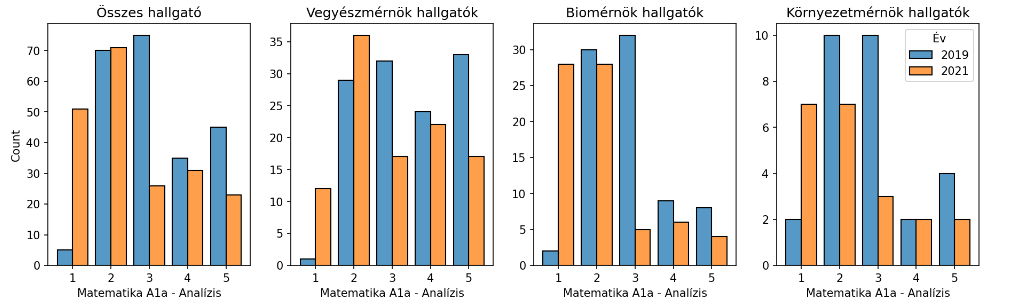
\includegraphics[width=\textwidth]{kepek/jegyek_eloszlas2.png}
\caption{Az elsőéves matematikajegyek eloszlása az egyes években}
\label{fig:jegyeloszlas}
\end{figure}

A legszembetűnőbb különbség a két év között az elégtelen, elégséges és közepes érdemjegyek eloszlásának tekintetében van. Az összesített ábrán jól látható módon míg 2019-ben a 2-es és 3-as érdmejegyek vannak túlsúlyban, addig 2021-ben az 1-es és 2-es érdemjegyek kerültek többségbe. Ugyanez a jelenség figyelhető meg a biomérnök és környezetmérnök hallgatók esetén is.

A \textit{seaborn pairplot} függvény előnye, hogy csak az általunk vizsgált változók oszlopait kell megadni, és az összes kombinációt egyszerre számítja ki és ábrázolja egy megfelelő méretű mátrixban. Először tekintsük a \textit{matplotlib figure} alakzatokba összesített ábrákat. Ezeknek az az előnye a \textit{seaborn pairplot}-tal szemben, hogy tetszőleges ábrákat lehet belehelyezni, így például színezéssel bevihető egy harmadik dimenzió a szórásdiagramba. Sőt negyedik dimenziót is lehetne ábrázolni a pontok kinézetének módosításával, de az már nehezen értelmezhető.

\begin{figure}[H]
\centering
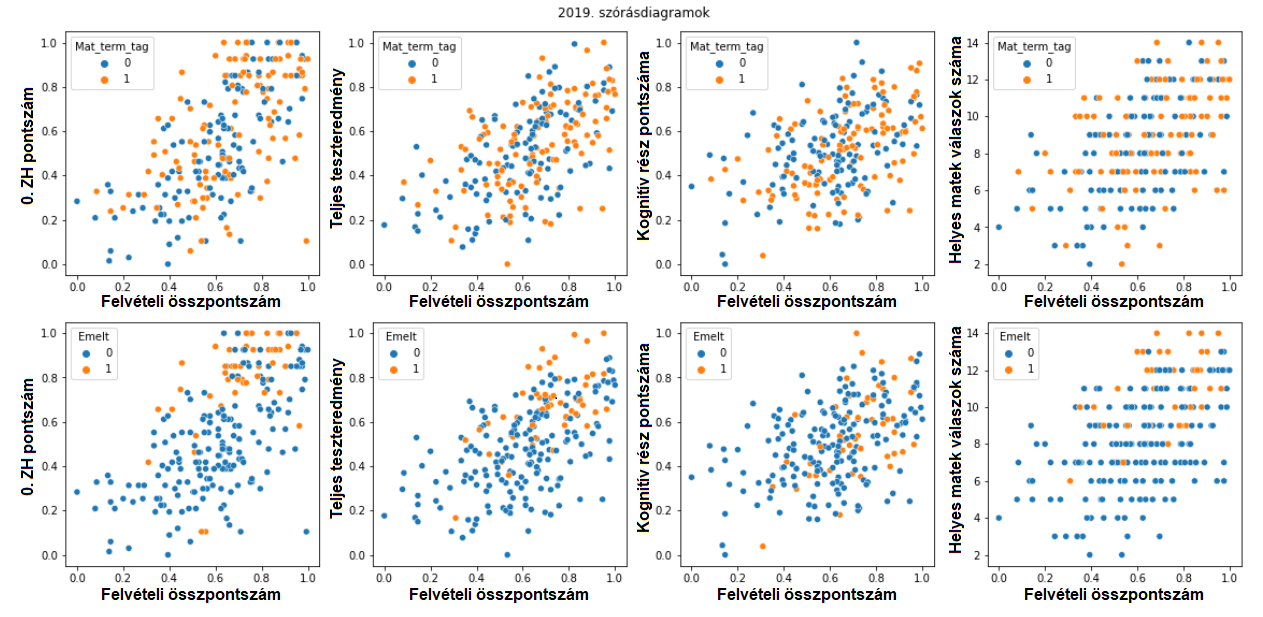
\includegraphics[width=\textwidth]{kepek/2019scatter.png}
\caption{2019. Szórásdiagramok}
\label{fig:2019scatter}
\end{figure}

A \ref{fig:2019scatter}. ábrán egyrészt a 0. ZH, a teszt összpontszáma és a két külön rész pontszámai vannak ábrázolva pontfelhőként a felvételi összpontszám függvényében, de minden eset kétszer. A felső sorban a pontok az alapján vannak színezve, hogy járt-e természettudományi tagozatra a hallgató (1 igen, 0 nem), az alsóban pedig, hogy emelt szinten érettségizett-e (1 igen, 0 nem).

Egyrészt rögtön látszik, hogy minden ábrán a bal felső és a jobb alsó sarkokban többnyire nincs pont, ez a pozitív korreláció, azaz összefüggés jele. Másrészt a színezésből arra következtethetünk, hogy az emelt érettségi megléte erősen fölfele húzza a többi eredményt, míg a természettudományi tagozatosok esetében nem egyértelmű a helyzet, drasztikus elkülönülés nincs.






\subsection{Folyamatábrák (Sankey-diagramok)}
A Sankey-diagramok olyan folyamatábrák, amelyekben az ábrázolt folyamok szélessége arányos a megfelelő folyamértékekkel. Ezáltal könnyen ábrázolhatóak adott állapotok közötti folyamok, illetve ezek egymással vett aránya. Egy hátránya van, hogy egy ábrán csak két osztálycsoport között olvashatjuk le az áramlásokat. Ha egy harmadik osztálycsoportot is belehelyezünk, és csak a másodikkal kötjük össze, akkor az első és a harmadik közötti vándorlások nem jelennek meg rajta. Emiatt lesz némi redundancia a lentebb ismertetett ábrákban.\\
Dolgozatunkban hat opciót vizsgáltunk a két évben az elérhető adatoknak megfelelően. Mindkét esetben az állapotok a hallgatók valamely eredményét jelentették, például felvételi pontszámot.
\begin{itemize}

\item 2019:

\begin{enumerate}
\item matematikai teszt 1.,2. és 3. részeiben helyesen megoldott feladatok száma.
\item kognitív teszt eredmény - \textit{A1} jegy - \textit{A2} jegy.
\end{enumerate}

\item 2019 és 2021:

\begin{enumerate}
\item tanulmányi hozott pontszám - érettségi pontszám - \textit{A1} jegy.
\item felvételi pontszám - nulladik ZH - kognitív teszt eredmény.
\item felvételi pontszám - kognitív teszt eredmény - \textit{A1} jegy - kumulált átlag.
\item felvételi pontszám - kognitív teszt eredmény - első féléves átlag - kumulált átlag.
\end{enumerate}

\end{itemize}

Az első két esetben csak a 2019-es évfolyamról volt adat. Az utolsó esetben 2021-ben megegyezett a kutatás idejében az első féléves és a kumulált átlag, így ennél az utóbbi értelemszerűen nem lett még egyszer beletéve.

A matematikai teszt részeinek eredményein és az \textit{A1}, \textit{A2} jegyeken kívül a többi változó folytonos volt, így szükség volt ezek diszkretizálására. Öt-öt osztály lett létrehozva minden esetben, de nem feltétlenül került mindegyikbe hallgató. Az átlagok kerekítve lettek, a felvételi, kognitív teszt és nulladik zh pontszámok ekvidisztáns módon lettek felosztva.

A \textit{felvételi pontszám - nulladik ZH - kognitív teszt eredmény} változatban a nulladik zh és a teszt eredményei nullától az elérhető pontszámig lettek felosztva 20\%-os lépésközökkel. Továbbá a felvételi pontszám a legalacsonyabb értéktől 500 pontig. A többi változat a kutatás későbbi szakaszában készült, így a folytonos mutatók az értékkészletük terjedelme szerint lettek felosztva, nem az elérhető pontszámok alapján.

Ezután \textit{for ciklus} használatával elkészültek a tranzíciós mátrixok. Ezen mátrixok \textit{i}-edik sorának \textit{j}-edik eleme azt mutatta, hogy az egyik változó \textit{i}-edik osztályában hány olyan hallgató volt, aki a másik változó \textit{j}-edik osztályába került. Ez a folyamok szélességének megadásához volt szükséges.

A \textit{plotly.graph\_objects} könyvtár \textit{go.Sankey} függvényével lettek elkészítve egyenként az ábrák. Minden esetben meg kellett adni számozva a kiinduló és beérkező állapotokat, így a középső csoportok mindkét listában szerepeltek. A program index alapján kapcsolta össze a két listából az állapotokat, továbbá kellett egy harmadik lista, amelynek a megfelelő indexű eleme a két állapot közötti folyam mérete. Ezen kívül a folyamokhoz és magukhoz az állapotokhoz is színeket kellett még rendelni, ismét egy-egy listában, figyelve az indexeket. 

Végül a kirajzolódott ábrát kellett még kézileg igazítani, ugyanis az eredmények csoportjai nem feltétlenül álltak megfelelő sorrendben a függőleges tengelyen, illetve azokban az esetekben, amikor nem volt mind az öt osztályban hallgató, egy-egy csoport átcsúszott egy másik eredmény oszlopába. Ezek nem okoztak gondot, ugyanis a csoport mozgatásával a hozzátartozó sávok automatikusan mozogtak együtt.

%IDE BE KELL ILLESZTENI A teszt-a1-a2 ábrát
\begin{figure}[H]
\centering
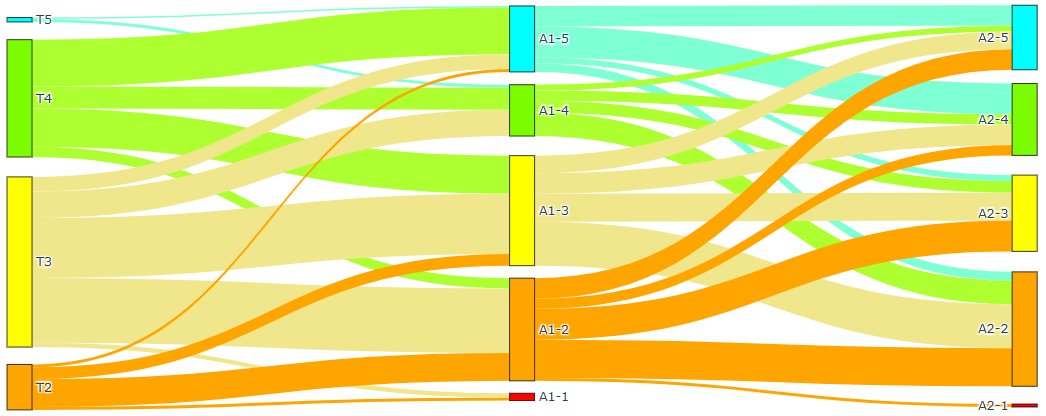
\includegraphics[scale=0.573]{kepek/teszt-a1-a2.png}
\caption{2019. Kognitív teszt eredmény - \textit{A1} jegy - \textit{A2} jegy}
\label{fig:teszt-a1-a2}
\end{figure}

A 2021-es gólyák a kutatás idejében még nem vehették fel az \textit{A2} tárgyat, így értelemszerűen csak a 2019-es évfolyamra készült ez az ábra.

Az ábrán rögtön látható, hogy a kognitív tesztben mindenki 20\% felett teljesített, de nagyon kevés hallgatónak sikerült 80\%-nál magasabb eredményt elérni. Ehhez képest az tantárgyakon elért jegyek eloszlása egyenletesebb. 

Látható, hogy akik a teszten gyengébben teljesítettek, azok a későbbiekben többnyire rosszabb jegyeket szereztek, de nem kevesen javítottak is. A jobban teljesítők szintén tartották általában a szintet, de itt sem elhanyagolható azok száma, aki rontott. Meglepő a kettesről négyes-ötösre javítók és az ötösről rosszabb jegyekre rontó hallgatók aránya a teljes viszonylatban.

Összességében sejthető, hogy egy hallgató teljesítménye a teszt során összefügg a további teljesítményével, de viszonylag sok esetben van jelentős romlás, illetve javulás.

%IDE BE KELL ILLESZTENI A matekrészeksankey ábrát
\begin{figure}[H]
\centering
\includegraphics[scale=0.573]{kepek/matekrészeksankey.png}
\caption{2019. Matematikai teszt 1. blokk - 2. blokk - 3. blokk helyes válaszok száma}
\label{fig:matekrészeksankey}
\end{figure}

A teszt matematikai részének a komplexitása a blokkonként nőtt, így érdekes volt megvizsgálni, hogyan teljesítettek a hallgatók, és hogyan viszonyul egymáshoz a helyes válaszaik száma a különböző blokkokban.

Rögtön látszik, hogy az első blokkban a hibátlan (négyes) osztály a legnagyobb, és a rosszabb eredmények száma csökken. Ez várható, hiszen itt alapismeretek voltak felmérve. A második és harmadik blokknál teljesen más a kép, a közepes osztályok körülbelül azonosak, a szélsők pedig kicsik, jobban hasonlít a normális eloszlásra.

A folyamok egészen változatosak. Az ábra közepén erősen szétoszlanak, de a széleihez közelítve kisebb trendek megfigyelhetők. Például a második blokkban minden kérdésre helyesen válaszolt hallgatók az első blokkban is többnyire szinte csak helyesen válaszoltak.

%IDE BE KELL ILLESZTENI A 2019_old_felvi_0zh_teszt ábrát
\begin{figure}[H]
\centering
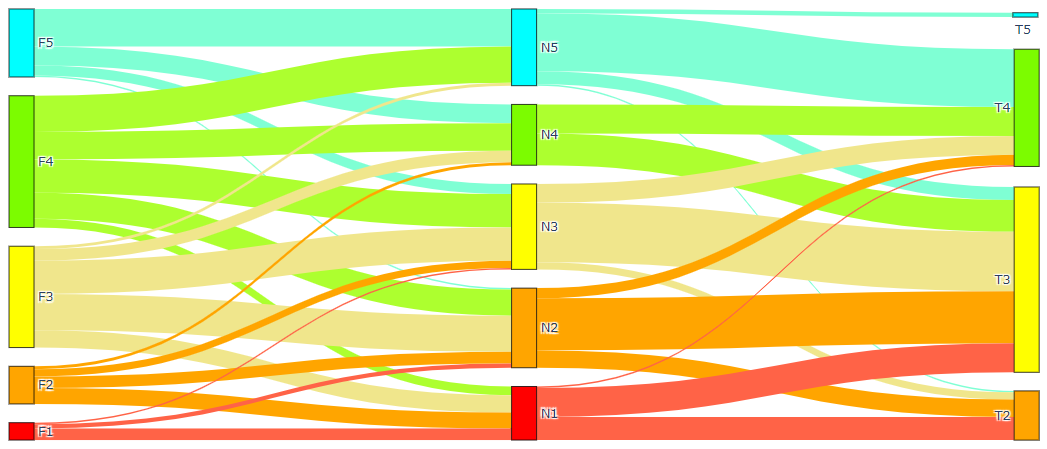
\includegraphics[scale=0.573]{kepek/2019_old_felvi_0zh_teszt.png}
\caption{2019. Felvételi - 0. zh - kognitív teszt pontszámok}
\label{fig:2019_old_felvi_0zh_teszt}
\end{figure}

Az ábrán főleg a 0. zh-ból a tesztbe menő folyamokon látszik egy erős tendencia. Igaz itt még a régebbi, teljes szerezhető pontszám szerinti felosztás van, így csak négy osztály jött létre, de nagyon kevés többosztálynyi ugrás van, tehát feltehető, hogy erősen összefügg a 0. zh és a kognitív teszt eredménye.

Ami a felvételi és 0. zh pontszámok kapcsolatait illeti, a folyamok egészen szerteágazóak, de itt is fennáll, hogy a közel hasonló teljesítmények között szélesebbek, mint a nagyobb különbségek esetén.

%IDE BE KELL ILLESZTENI A 2021_old_felvi_0zh_teszt ábrát
\begin{figure}[H]
\centering
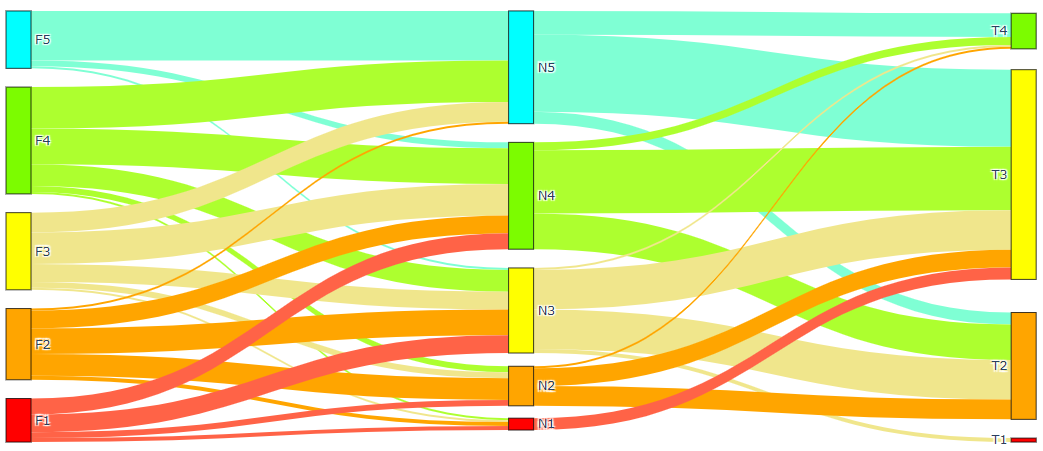
\includegraphics[scale=0.573]{kepek/2021_old_felvi_0zh_teszt.png}
\caption{2021. Felvételi - 0. zh - kognitív teszt pontszámok}
\label{fig:2021_old_felvi_0zh_teszt}
\end{figure}

Annak ellenére, hogy a tesztes oszlop a 2019-es tesztes oszlopra hasonlít, csak fejjel lefelé, ez a valós eloszlás. Valóban, míg 2019-ben nem volt 20\% alatti eredmény, itt fordítva, nem volt 80\% fölötti. A felvételi pontszámok arányai romlottak, arányosan nagyobbak lettek az alsó osztályok. Ellenkezőleg a 0. zh eredményei javultak, nagyobbak a magasabb pontszámhoz tartozó osztályok arányai. 

Ami a folyamokat illeti, többnyire hasonlóak a tendenciák, bár érdekes, hogy akiknek a legrosszabb lett a 0. zh, a kognitív teszt közepesen ment. Itt is mondható, hogy a jobban teljesítő hallgatók többnyire mindenből jól teljesítettek, illetve a gyengébbek között ritkábbak voltak a jobb eredmények. Ennek ellenére itt is szerteágazóak a folyamok, tehát összefüggés van, de nem nagyon erős.


%IDE BE KELL ILLESZTENI A 2019_felvi_teszt_atlag_kumatlag ábrát
\begin{figure}[H]
\centering
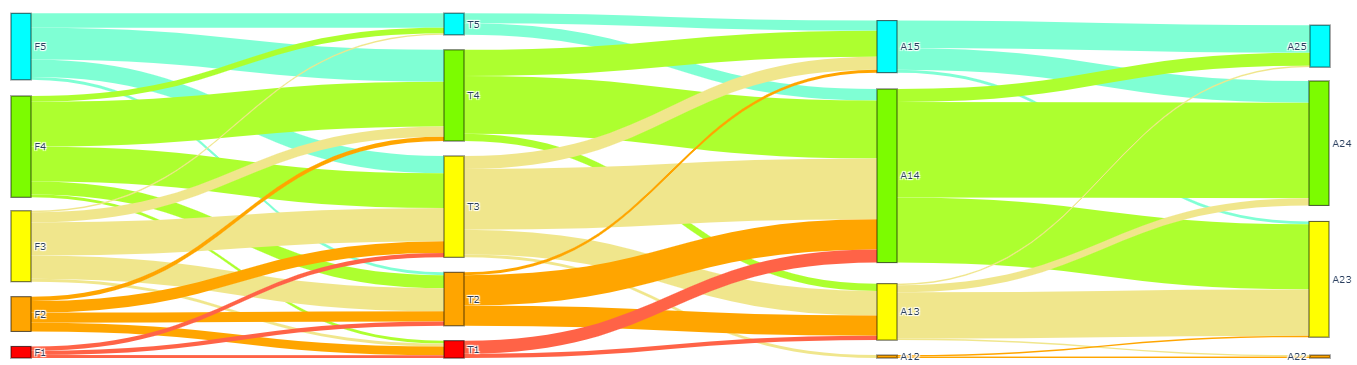
\includegraphics[scale=0.6]{kepek/2019_felvi_teszt_atlag_kumatlag.png}
\caption{2019. Felvételi - kognitív teszt pontszám - első féléves átlag - kumulált átlag}
\label{fig:2019_felvi_teszt_atlag_kumatlag}
\end{figure}

Ezen az ábrán már közvetlenül láthatóak a felvételi és kognitív teszt eredményeinek viszonyai, azonban itt már az értékkészlet van felosztva ekvidisztánsan. Ez abban is megnyilvánul, hogy a teszt pontszámosztályainak mások az arányai. 

Két előnye volt az értékkészlet szerinti osztályozásnak: gyorsabb volt (egy függvényre volt csak szükség), illetve így az eredmények egymáshoz képest való relatív eloszlása jobban látszik. Míg a régebbi ábrán nagyon nagy a hármas osztály, mert a legtöbben 40-60\% körüli eredményeket értek el, itt az látszik, hogy a legjobb és legrosszabb dolgozatok pontszámai között, a terjedelem 20\%-ával lépkedve milyen a hallgatók eloszlása. Így az lesz valóban "középtájban", aki a többi hallgató pontszámához képest átlaghoz közeli pontszámot szerzett, nem pedig az a sok tanuló, aki 40-60\%-ot ért el.

Visszatérve az ábrára, a fentebb megfigyelt tendenciák lényegében ismétlődnek, jó eredményeket jók, rosszakat rosszak követik nagyrészt, de továbbra is változatosak a folyamok. Összefüggőség szempontjából jó jel, hogy a legjobb teszteredményt elérők négyesnél rosszabb átlagot nem értek el. Sőt nagyon sok hallgatónak volt négyes az átlaga az első félévben, ami nagyrészt kétfelé oszlott az idő elteltével, többen megtartották, de sokan rontottak hármasra, páran javítottak. A többi átlagértékkel hasonló a helyzet, inkább megmaradt, mint javult vagy romlott.

%IDE BE KELL ILLESZTENI A 2021_felvi_teszt_atlag ábrát

\begin{figure}[H]
\centering
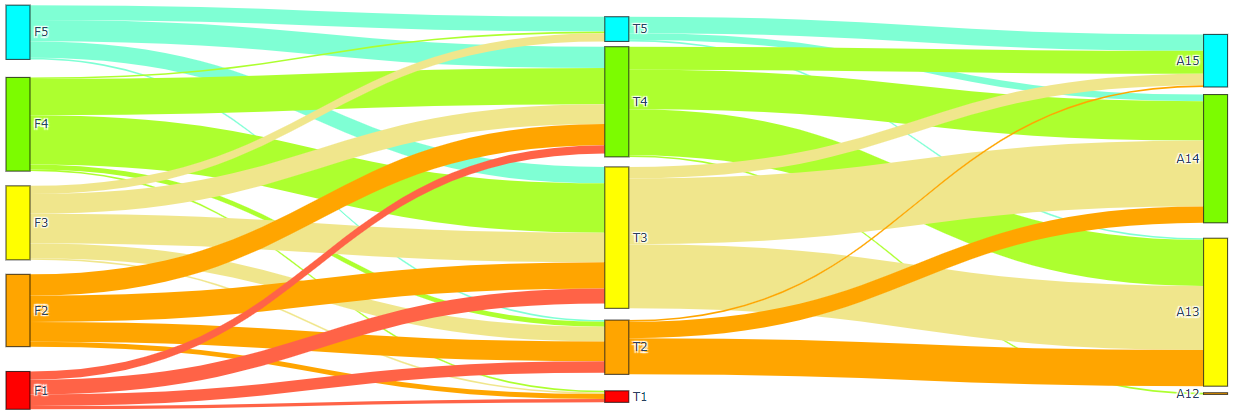
\includegraphics[scale=0.6]{kepek/2021_felvi_teszt_atlag.png}
\caption{2021. Felvételi - kognitív teszt pontszám - első féléves átlag}
\label{fig:2021_felvi_teszt_atlag}
\end{figure}

A kutatás során ez az évfolyam még az első évében volt, így csak első féléves átlagokról volt adatunk. Ettől eltekintve 2019-hez képest több hallgatónak volt relatíve gyengébb a felvételi pontszáma, de ennek megfelelően többen is "javítottak". Az átlagok eloszlása romlott, aránylag több hármas és kevesebb négyes, illetve ötös lett. 

%IDE BE KELL ILLESZTENI A 2019_felvi_teszt_a1_kumatl ábrát
\begin{figure}[H]
\centering
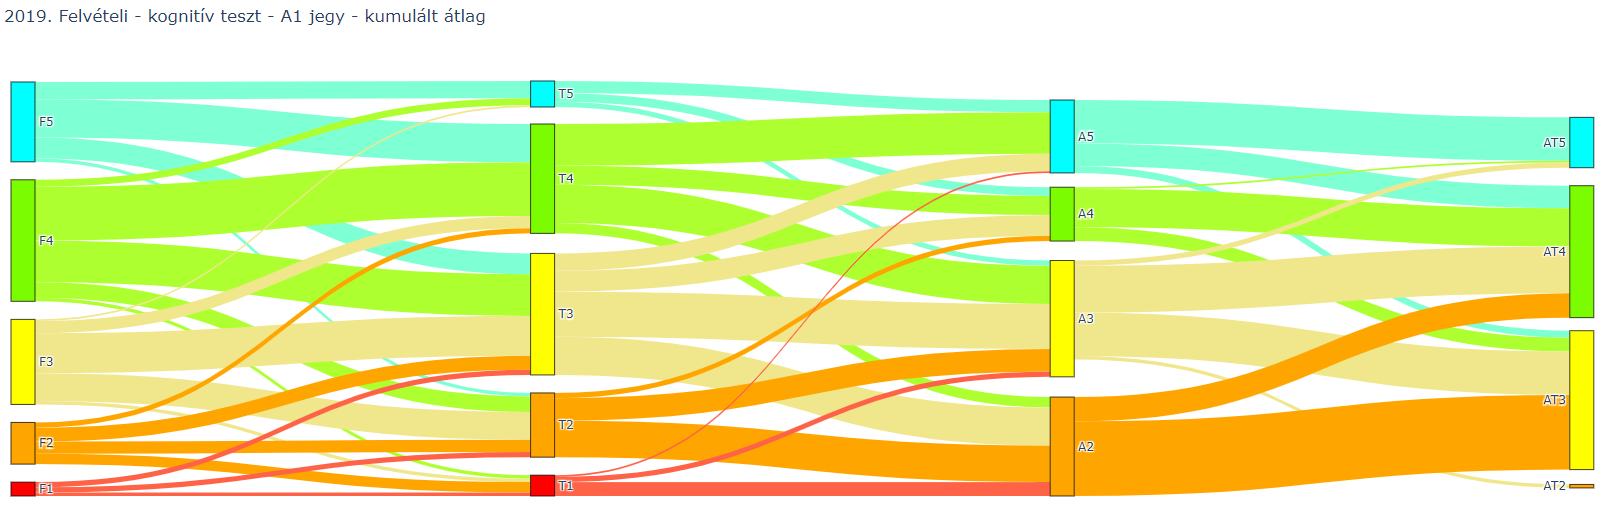
\includegraphics[scale=0.5]{kepek/2019_felvi_teszt_a1_kumatl.png}
\caption{2019. Felvételi - kognitív teszt pontszám - \textit{A1} jegy - kumulált átlag}
\label{fig:2019_felvi_teszt_a1_kumatl}
\end{figure}

Az első két oszlop viszonyát már láttuk, az újdonság az \textit{A1} jegy az első féléves átlag helyett. Ettől függetlenül a tendenciák változatlanok, azok szereztek jobb, illetve rosszabb jegyet, akik rendszerint jobban, illetve rosszabban írták meg a tesztet. A trendet továbbra erősíti a jegyek és átlagok viszonya, bár értelemszerűen nem meglepő, hogy a két dolog összefügg.

%IDE BE KELL ILLESZTENI A 2021_felvi_teszt_a1_atlag ábrát
\begin{figure}[H]
\centering
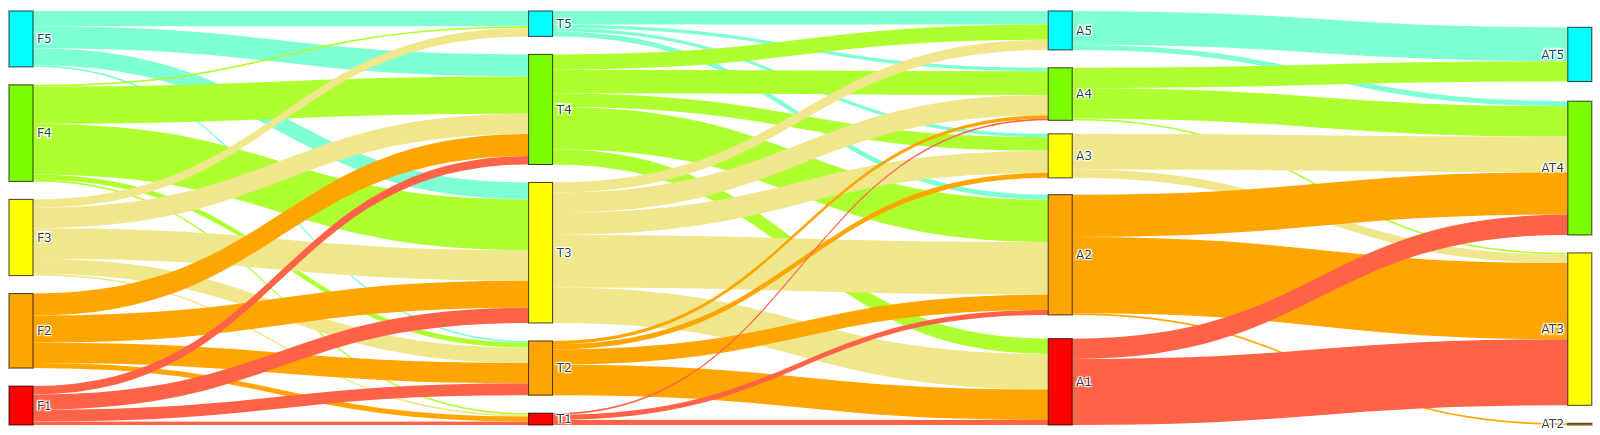
\includegraphics[scale=0.5]{kepek/2021_felvi_teszt_a1_atlag.png}
\caption{2021. Felvételi - kognitív teszt pontszám - \textit{A1} jegy - első féléves átlag}
\label{fig:2021_felvi_teszt_a1_atlag}
\end{figure}

Szembetűnő, hogy az \textit{A1} jegyek valamilyen okból kifolyólag erősen romlottak. Míg 2019-ben nem bukott egy hallgató sem, itt majdnem a csoport negyedének nem sikerült elvégezni a tárgyat, sőt olyanoknak is, akik a legjobbak között voltak a teszt alapján. Továbbá a csoportnak több, mint a fele nem tudott kettesnél jobb jegyet szerezni. Fentebb láttuk, hogy az átlagok is romlottak, de ezek szerint nem olyan mértékben, mint az \textit{A1} jegyek. Érdekes, hogy az egyest és kettest szerzett hallgatók mégis nagyrészt hármas, sőt nem kevesen négyes átlagot szereztek. Ettől függetlenül a szokásos trendek itt is megmutatkoznak.
 
%IDE BE KELL ILLESZTENI A 2019_hozott_erett_A1 ábrát
\begin{figure}[H]
\centering
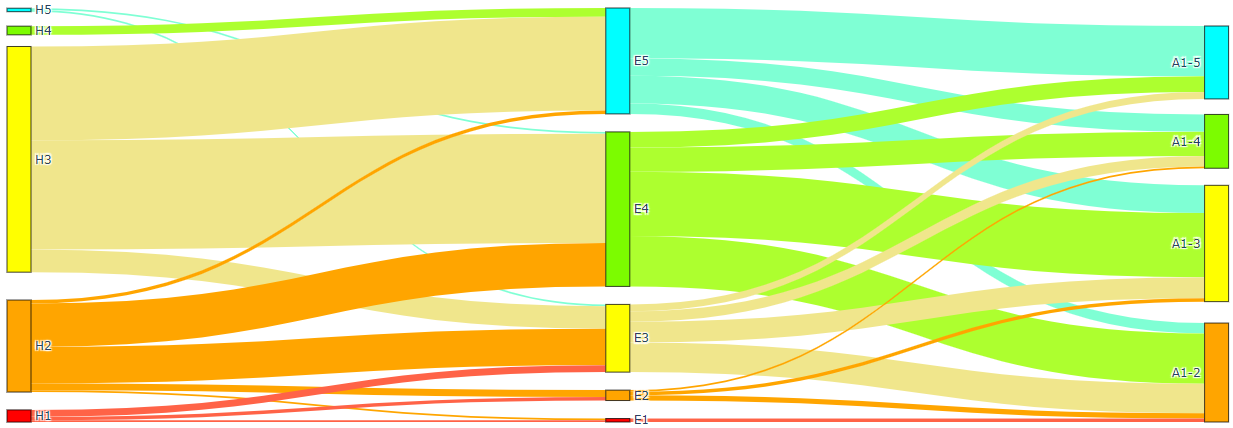
\includegraphics[scale=0.6]{kepek/2019_hozott_erett_A1.png}
\caption{2019. Hozott és - érettségi pontszám - \textit{A1} jegy}
\label{fig:2019_hozott_erett_A1}
\end{figure}
Ahogy később látni fogjuk, a modellek alapján a hozott és érettségi pontszámok erősen befolyásolták a jegyekre vett predikciókat, így utólag elkészült ez és a következő ábra.

Jellegzetes, hogy a hallgatók nagy részének hasonló volt a hozott pontszáma, nagyon kevésnek volt kiemelkedő vagy relatíve kicsi. Aránylag kevés hallgatónak volt a legjobb pontszám 60\%-a alatt az érettségije. Még ezek mellett is megőrződött az a tendencia, hogy egy-egy hallgató nagyrészt hasonlóan teljesít a különböző mutatók alapján.

Az ábráról leolvasható, hogy míg az utolsó oszlop felső felébe szinte csak kék és zöld folyamok érkeznek, mégis szerteágaznak, és például a legjobb érettségi pontszámokkal rendelkezők közül is többen kettest szereztek a tárgyból. 

%IDE BE KELL ILLESZTENI A 2021_hozott_erett_A1 ábrát
\begin{figure}[H]
\centering
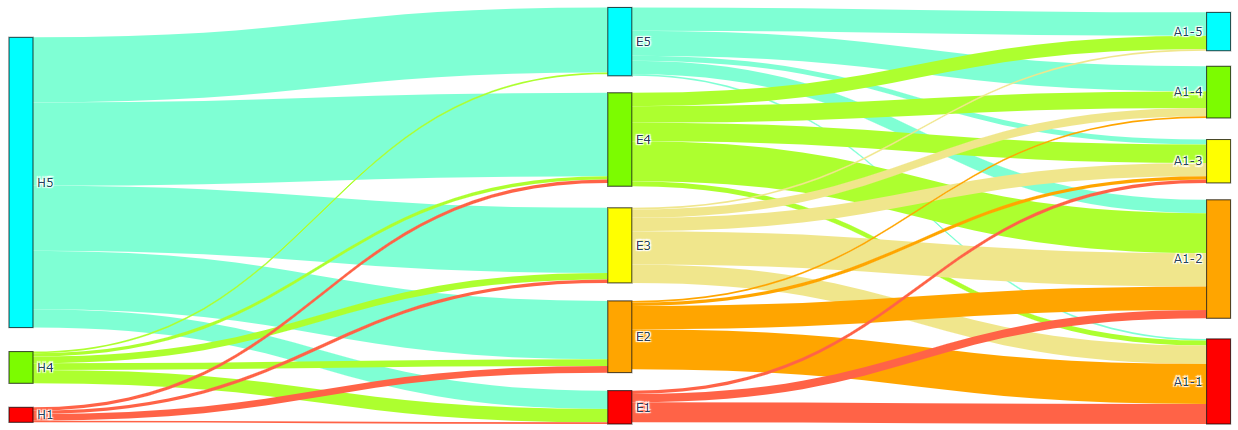
\includegraphics[scale=0.6]{kepek/2021_hozott_erett_A1.png}
\caption{2021. Hozott és - érettségi pontszám - \textit{A1} jegy}
\label{fig:2021_hozott_erett_A1}
\end{figure}

Az ábrán rögtön szembetűnik egy meglepő dolog, a hozott pontszámoknál van egy óriási ötös osztály. Az értékeket leellenőrízve, tényleg nagyon sok esetben 180 és 190 között mozgott a hozott pontszám.

Ehhez, és a 2019-es ábrához képest az érettségi pontszám viszont egészen egyenletesen oszlott el. Az ábra bal felétől eltekintve, a teljesítmény megmaradására vonatkozó tendencia igaz gyengébben, de ismét jelen van.


\subsection{Klaszterezés}

EZ MÉG CSAK RÁVEZETÉS

-----------

Cél: gép által csoportosítani a hallgatókat több változó alapján, keresni jó magyarázó változókat, hogy egyszerűsíthető legyen a csoportosítás.

Változók: összesített teszteredmény, külön matek/kognitív eredmény, első félév átlaga, kumulált átlag, felvételi pontszám összesítve és részekre bontva. Ezen attribútumok nem redundáns részhalmazai.
	Az algoritmusok hatékonyabb és gyorsabb működése érdekében a változók értékei normalizálva és skálázva lettek. Három-három táblázat készült a 2019, 2020, 2021 évekre: min-max, illetve kvantilis szerint skálázott, továbbá standardizált értékekkel.
	Három klaszterező algoritmus lett alkalmazva a legjobb eredmény elérése érdekében: K-közép, DBSCAN és Ward féle hierarchikus klaszterező algoritmus.
	Ezek futtatása előtt el lett végezve egy felderítő ábrázolás, amely nehézségekre hívta fel a figyelmet. Az adatok kétdimenziós vetületeit ábrázoltuk szórásdiagramokon. A pontfelhők között nem volt olyan, amelyen látványosan el lehetett volna különíteni egyes csoportokat, ami a klaszterezést nehezítette.

------------

\newpage
\section{Prediktív analitika}

\subsection{Modellek és metodológia}

Következő lépésként azt vizsgáltuk, hogy a két évben külön a bemeneti adatok alapján mennyire pontosan lehet előrejelezni egyes teljesítménymutatók értéket, illetve hogy a predikciókra nézve a különböző bemeneti változók, más néven attribútumok milyen és mekkora szereppel bírnak. Ehhez többféle modellen többféle \textit{gépi tanuláson alapuló osztályozó algoritmus} használatára volt szükség. A kutatás során kétféle eredmény alaposabb vizsgálatára összpontosítottunk mindkét évben: a "Matematika A1a - Analízis" tárgyból kapott érdemjegyre illetve az első félév végén megállapított kumulált tanulmányi átlagra. Ezen feladatok a felügyelt gépi tanulási problémák közé esnek, ahol a kitüntetett célváltozót szeretnénk a többi bemeneti változóval előrejelezni. Ekkor a gépi tanulás során a teljes adathalmazt tanító és teszthalmazra bontjuk, a tanító adathalmazon betanítjuk az algoritmusokat úgy, hogy a tanítóhalmazbeli adatok célváltozóját minél pontosabban prediktálják, majd valamilyen metrika szerint kiválasztjuk a betanított algoritmusok közül a legjobbat. A legoptimálisabb osztályozó kiválasztásához többnyire \textit{keresztvalidációt} alkalmazunk. Keresztvalidáció során a tanítóhalmazt felbontjuk K egyenlő részre, melyek közül az egyiket kinevezzük validációs halmaznak. Ezt követően az algoritmusokat betanítjuk a maradék $K$-$1$ részen, amelyeket aztán a validációs halmazon kiértékelünk. Ezt összesen $K$ alkalommal ismételjük, mindig másik részt választva validációs halmaznak, majd azt az algoritmust dedikáljuk a legjobbnak, amelynek az aggregált teljesítménye a $K$ darab iteráció során a legjobb. Az így kapott osztályozót még visszamérjük a teszthalmazon is az általánosítóképesség ellenőrzése végett. A kutatás során a cél a teszthalmazon való minél hatásosabb előrejelzés mellett az egyes éveknél használt és optimalizált algoritmusok esetén a különböző attribútumok prediktív erejének összehasonlítása volt.

A két vizsgált probléma közül az előbbi alapvetően egy osztályozási probléma öt osztállyal, míg az utóbbi egy regressziós feladat. Az előbbi feladathoz ötféle algoritmust, \textit{Gradient Tree Boosting-ot, Naive Bayes-t, logisztikus regressziót, SVM-et} és \textit{lineáris regressziót} használtunk, az utóbbihoz lineáris regressziót és Gradient Tree Boosting-ot (ezen algoritmusok működése és optimalizálása a következő fejezetben lesz ismertetve). Azért esett a választás ezen algoritmusokra, ugyanis számos egyetemi teljesítményt és lemorzsolódást vizsgáló tanulmány során teljesítettek kiváló eredménnyel. (IDE REFERENCIÁK) Mivel azonban viszonylag kevés adat állt a rendelkezésünkre, ezért az érdemjegyek prediktálásánál az adatrekordok esetén a pontos érdemjegy helyett érdemjegy csoportok előrejelzésére koncentráltunk. A matematika érdemjegycsoportok prediktálására így kétféle modell került felvázolásra: egy \textit{3 csoport modell}, illetve egy \textit{2 csoport modell}.

A 2 csoport modell esetén a két csoportot a \{5,4,3\} illetve \{2,1\} osztályok adják, míg a 3 csoport modellnél az osztályok \{5,4\}, \{3,2\} illetve \{1\} módon alakultak. Az előbbi esetben az osztályok intuitívan a lemorzsolódási veszélyeztetettség szerint formálódtak, míg az utóbbiban egy általánosabb "jól teljesítő", "rosszul teljesítő", "lemorzsolódott" csoporthármast kívántunk elérni. Mindkét modell esetén külön vizsgáltuk a teljesítményt összes hallgatóra vonatkozóan illetve szétbontva vegyészmérnök és biomérnök hallgatókra egyaránt (a környezetmérnökökről nem állt rendelkezésre elég adat, így őket a szakonkénti bontásban kihagytuk).

A használandó osztályozó algoritmusok közül a Naive Bayes és Gradient Tree Boosting algoritmusok képesek kezelni a többosztályos feladatokat, a lineáris regresszió azonban folytonos célváltozóérték prediktáláshoz használható, így ott a prediktált értéket kerekítettük a legközelebbi címkeértékhez, a logisztikus regresszió és az SVM pedig alapjáraton csak bináris osztályozásra alkalmas, így a náluk \textit{One-vs-Rest} elvű osztályozást használtunk. Az elv lényege, hogy minden osztály esetén képezünk egy új virtuális osztályt, amely az összes többi osztályt tartalmazza, majd minden ilyen osztálypár esetén a bináris osztályozó meghatározza a kérdéses adatrekord esetén az osztályba tartozási valószínűségeket. Végül azt a címkét prediktáljuk a rekordnak, amely osztály esetén a legnagyobb ez a valószínűség. 

Az egyes modellek és almodellek esetén a tanítás előtt főkomponens analízist (Principal Component Analysis) is alkalmaztunk. Az eljárás lényege, hogy az adatpontokat egy kisebb dimenziós térre vetítjük le oly módon, hogy a változók közötti varianca minél nagyobb részét tartsák meg, így minimalizálva az információveszteséget. Az új változók, amelyeket főkomponensnek nevezünk, a kisebb dimenziós térben az eredeti változók kovarianciamátrixának sajátvektorai lesznek. PCA használata során az algoritmusok gyorsabban tanulnak a kisebb dimenziószám miatt, és olykor jobb eredményt is érnek el. Jelen kutatásban másrészt azért is döntöttünk a PCA alkalmazása mellett, mert a korábbi, ugyanezen problémakört vizsgáló, általunk átnézett tanulmányok nem használtak PCA-t még nagyobb attribútum szám esetén sem, ugyanakkor mi a korai tanító-tesztelési fázisnál azt tapasztaltuk, hogy az áttranszformált adatokon jobban teljesítenek az osztályozó algoritmusok, így potenciálisan megéri alkalmazni.

\subsubsection*{Implementálás}

A \textit{jegycsoportok} prediktálására épített modellezési struktúrát \ref{fig:modell}. ábra mutatja. Valamennyi csoportmodellnél a teljes adathalmazt felbontottuk tanító- és teszthalmazra 70-30 arányban, majd a tanítóhalmazra illesztett PCA modellt alkalmaztuk a teszthalmazra is, ahol a főkomponensek számát minden modellnél 2 és 8 között iterálva változtattuk 2-es lépésközzel. Ezt követően a változókat kvantilis alapú 0-1 skálázásnak vetettük alá, ahol az algoritmusok jobb teljesítőképessége és a változók kiértékelés utáni összehasonlíthatósága végett a különböző attribútumok értékeit a kvantilisek mentén a $[0, 1]$ intervallumba transzformáltuk át, valamint az érdemjegy csoportok prediktálásához a 2 és 3 csoport modelleknél a célváltozó-értékeket rendre 1, 0-ra illetve 3, 2, 1-re módosítottuk. 

\begin{figure}[h]
\centering
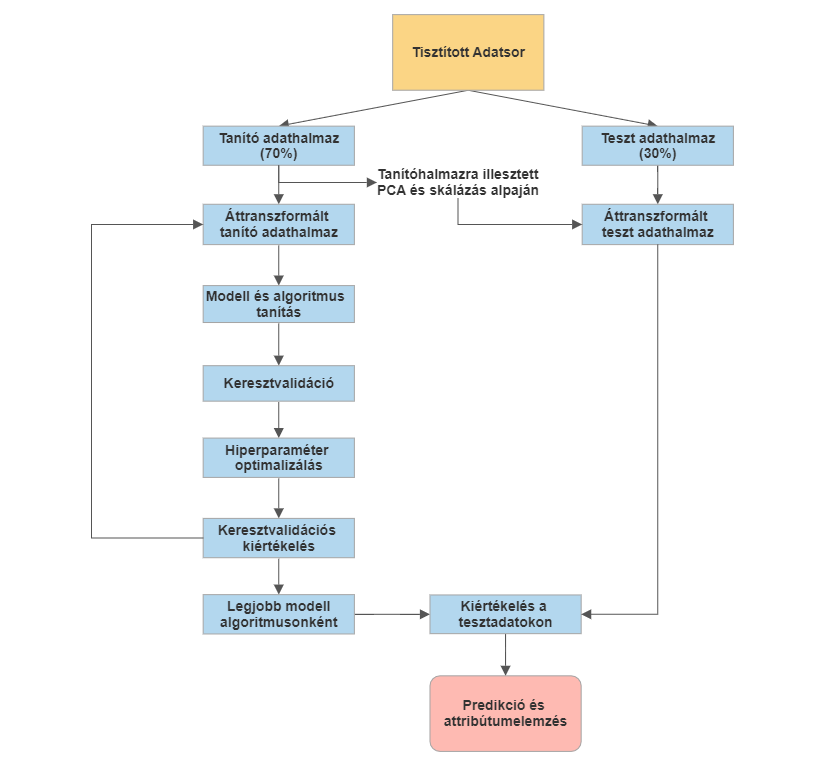
\includegraphics[scale=0.6]{kepek/flowchart.png}
\caption{A modellezési struktúra sematikus ábrája}
\label{fig:modell}
\end{figure}

Valamennyi algoritmus hiperparamétereinek optimális megválasztására 5-szörös keresztvalidációt alkalmaztunk, ahol törekedtünk arra, hogy az adatrekordok címkéjének eloszlása egyenletes legyen a felosztott részek között. A keresztvalidációnál használt, jóságot mérő metrikának a kiegyensúlyozott pontosságot ('\textit{balanced accuracy}') választottuk, amelynek képlete az alábbi:
\begin{align*}
\text{balanced-accuracy} = \frac{1}{2}\left(\frac{TP}{TP+FN} + \frac{TN}{TN+FP} \right) 
\end{align*}Ezen metrika alapvetően bináris, pozitív-negatív osztályú osztályozási problémákhoz alkalmas, de többosztályos osztályozás esetén is használható, ahol az egyes osztályokhoz tartozó \textit{TP, FP, FN, TN} értékek által kiszámított kiegyensúlyozott pontosságok számtani közepét nézzük. A képlet egyes jelölései 2 valamint több osztály esetén:  \\ \\
- \textbf{TP} a pozitívnak (osztálybelinek) osztályozott, valóban pozitív (osztálybeli) adatrekordok száma \\
- \textbf{FP} a pozitívnak (osztálybelinek) osztályozott de valójában negatív (nem osztálybeli) adatrekordok száma \\
- \textbf{FN} a negatívnak (nem osztálybelinek) osztályozott de valójában pozitív (osztálybeli) adatrekordok száma \\
- \textbf{TN} a negatív (nem osztálybelinek) osztályozott, valóban negatív (nem osztálybeli) adatrekordok száma \\ 
\\
A választott metrika mellett meghatároztuk a legjobb algoritmusokat, amelyeket a teszthalmazon visszamértünk, valamint kiértékeltük az ily módon választott modellek esetén az egyes változók fontosságát is.

A \textit{kumulált átlag} predikciójánál a tisztított adathalmazt ugyanúgy 70-30 arányban osztottuk fel. Adattranszformálásra csak skálázást alkalmaztunk, PCA-t nem, majd valamennyi osztályozó hiperparamétereinek optimalizálása hasonlóan 5-szörös keresztvalidációval történt. Az illesztett modellekkel mindkét évben feljegyeztük az $R^2$, $MAE$ (átlagos abszolút eltérés) és $RMSE$ (gyököt vont átlagos négyzetes eltérés) statisztikákat, a reziduális tagok szórásdriagramját, illetve az egyes változók prediktív erejét.





%TODO: Recall definícióját ismertetni?

\subsection{Osztályozó algoritmusok és optimalizálásuk}

(ez a szekció még félkész)

\subsubsection{Lineáris regresszió}

A lineáris regresszió jellegéből adódóan alapvetően folytonos célváltozó prediktálására alkalmas, ugyanakkor kategorikus, ordinális címkéjű adatok osztályozására is fel lehet használni. Az algoritmus lényege, hogy a magyarázóváltozók mindegyikéhez egy-egy súlyt rendelünk, majd az adatpont attribútumértékeinek vesszük a súlyokkal való súlyozott összegét, és esetleg egy bias tagot hozzáadva az így kapott szumma lesz a prediktált címkeérték. A cél a tanítás során a súlyok optimális megtalálása, miközben a tanítóhalmazon minimalizáljuk a célváltozóérték és a prediktált érték közötti négyzetes hibát.

Mivel az algoritmus implementálása során a legkisebb négyzetek elvét alkalmazza, amellyel az optimális megoldás analitikusan elérhető, ezért nem történt hiperparaméter-optimalizáció.

\subsubsection{Naive Bayes}

%A Naive Bayes azon tényből indul ki, hogy a minimális osztályozási hibát akkor kapjuk, ha minden adatrekordhoz azt a $c$ címkét rendeljük, amelyre a $\mathbb{P}(C=c|\underline{X} = \underline{x})$ feltételes valószínűség maximális, ahol $\underline{X}=(X_1,X_2, \dots ,X_k)$ jelöli az attribútumokat, $\underline{x} = (x_1, x_2, \dots , x_k)$ az adatrekordhoz tartozó attribútumvektort, $C$ pedig a célváltozót. Vagyis a keresett optimális $c^*$ címkére az alábbi teljesül:
%\[
%c^* = \argmax_c \mathbb{P}(C=c|\underline{X} = \underline{x})
%\]
%
%Ez a Bayes-tétel és a teljes valószínűség tétele segítségével az alábbi formára hozható:
%\[
%c^* = \argmax_c \mathbb{P}(\underline{X} = \underline{x}|C=c) \cdot \mathbb{P}(C=c)
%\] 
%A Naive Bayes algoritmus naívan azzal a feltételezéssel él, hogy az attribútumok a célváltozó ismeretében feltételesen függetlenek, így ekkor a feltételes valószínűség felbontható szorzatra:
%\[
%\mathbb{P}(\underline{X}|C) = \mathbb{P}(X_1|C) \cdot \mathbb{P}(X_2|C) \cdot \dots \cdot \mathbb{P}(X_k|C)
%\]
%
%Ekkor a $\mathbb{P}(X_i=x_i|C=c_j)$ és $\mathbb{P}(C=c_j)$ valószínűségeket a tanító adatokból már meg tudjuk becsülni:
%\begin{align*}
%\mathbb{P}(X_i=x_i|C=c_j) &= \frac{n_{ij}}{n_j} \\
%\mathbb{P}(C=c_j) &= \frac{n_j}{n}
%\end{align*}
%ahol: \\
%- $j$ a lehetséges címkék száma, $n$ az összes tanító adatrekord száma.  \\
%- $n_{ij}$ azon tanító adatrekordok száma, amelynek $i$-edik attribútuma $x_i$ és a címkéje $c_j$. \\
%- $n_j$ pedig a $c_j$ címkéjű tanító adatrekordok száma. \\


A Naive Bayes algoritmus működése mögött álló alapelv az, hogy feltesszük az attribútumok feltételes függetlenségét, amennyiben a célváltozó értéke ismert. Osztályozás során azt vizsgáljuk, hogy mely címkeérték mellett a legnagyobb a valószínűsége annak, hogy az adott adatrekord attribútumai éppen a felvett értékeket kapták. A megfelelő valószínűségeket a tanítóhalmazbeli adatok attribútumértékeinek különböző címkék melletti relatív gyakoriságai adják. 

Az algoritmus a jellegéből adódóan nem igazán optimalizálható, így a Naive Bayes esetén nem történt keresztvalidáció.

\subsubsection{Gradient Tree Boosting}

A Gradient Boosting algoritmus egy Ensemble típusú osztályozó, amelyek lényege, hogy sok gyenge teljesítményű prediktor (\textit{"weak learner"}) eredményét felhasználva hoz egy erős predikciót. Gradient Tree Boosting esetén a gyenge prediktorok \textit{döntési fák}, amelyek lefelé irányított, legtöbbször bináris fák, amelyeknek minden belső csúcsában egy attribútumra vonatkozó feltétel szerepel, a levelei pedig valamilyen célváltozóértékkel címkézettek. A boosting eljárás során minden fázisban egy új döntési fát építünk, amely megpróbálja az előző fázisban épített fa hibáit csökkenteni az úgynevezett reziduálisokra építve. A cél egy erős prediktorként funkcionáló döntési fa létrehozása ráerősítések sorozata révén. (REFERÁLNI FRIEDMAN CIKKÉT)

%Legyen $F_{m-1}$ az $m$-$1$-edik fázisban kapott modell, majd jelölje $h_m(x)$ az $m$-edik fázisban épített döntési fát. Jelölje $J_m$ ennek a fának levélszámát illetve jelölje $R_{1m},\cdots,R_{J_mm}$ a bementi adatok terének egy felosztását a levelek alapján. 


A keresztvalidálás során optimalizált paraméterek: \\
- Tanulóráta (0.01 és 5 között változtatva 0.1-es lépésközzel)\\
- Boosting fázisok száma (5 és 100 között változtatva 5-ös lépésközzel)\\
- Facsúcsokban használt vágási feltétel (négyzetes hiba, Friedman MSE) \\

\subsubsection{Logisztikus regresszió}

%A logisztikus regresszió nevéből adódóan egy regressziós algoritmus, tehát folytonos célváltozóértéket prediktál, azonban bináris osztályozásra használják. Alapja a \textit{szigmoid} függvény, amelynek értelmezési tartománya a valós számok halmaza, értékkészlete pedig a $(0,1)$ intervallum.
%%\begin{minipage}{•}
%\begin{align}
%\sigma(z) = \frac{1}{1+e^{-z}}
%\end{align}
%%\end{minipage}
%Legyen az $n$ darab tanító adatunk $(\underline{x}_1,y_1),(\underline{x}_2,y_2), \dots , (\underline{x}_n,y_n)$, ahol \\ $\underline{x}_i=(x_{i1},x_{i2}, \dots , x_{ik})$ az $i$-edik tanítóadat $k$ hosszú attribútumvektora, $y_i$ pedig az ehhez tartozó célváltozóérték. A cél az, hogy olyan $\underline{w} = (w_1,w_2, \dots , w_k) \text{ és } b$ súlyokat találjunk, amelyek esetén az összesített hiba értéke minimális. Egy adatrekord esetén a logaritmikus hiba adott súlyokkal:
%\begin{align}
%cost_{w,b}(\underline{x}_i) =  -y_i\log \left( \sigma(\underline{w}^T\underline{x}_i+b) \right) -(1-y_i)\log(1-\sigma(\underline{w}^T\underline{x}_i+b))
%\end{align}
%Az összes adatrekordra vonatkozó, végcélként minimalizálandó hibafüggvény pedig az alábbi:
%
%\begin{align}
%C(\underline{w},b) = -\frac{1}{n}\sum_{i = 1}^n \left( y_i\log \left( \sigma(\underline{w}^T\underline{x}_i+b) \right) +(1-y_i)log(1-\sigma(\underline{w}^T\underline{x}_i+b))\right)
%\end{align}
%
%Sok esetben ez a hibafüggvény még kiegészül egy $\lambda||(\underline{w},b)||^2$ ( ahol$||(\underline{w},b)||$ a \\ $(w_1,w_2, \dots , w_k, b)$ súlyvektor hossza) \textit{regularizációs taggal}, amely segít megakadályozni azt, hogy egyes súlyok túl nagy értéket vegyenek fel, így megelőzve a túltanulást. Itt $\lambda$ az állítható, valós \textit{regularizációs hiperparaméter}, amelyet minél nagyobbra állítunk, annál jobban bünteti a túltanulást.
%
%Ha a $k$ hosszú attribútumvektorainkat egy $k$-dimenziós tér pontjaiként fogjuk fel, a logisztikus regresszió ezekkel a súlyokkal lényegében egy optimális, lineárisan szeparáló $\underline{w}^T\underline{x}+b=0$ hipersíkot keres. Ha az $i$-edik adatrekordra $\underline{w}^T\underline{x}_i+b>0$, akkor azt pozitív 1-es  osztályba sorolja, ha pedig $\underline{w}^T\underline{x}_i+b<0$ akkor pedig a negatív 0-ás osztályba sorolja az osztályozó. A keresztvalidálás során optimalizált paraméterek: \\
%- Regularizációs paraméter (0.05 és 5 között változtatva 0.05-ös lépésközzel) \\
%- Önoptimalizálási módszer ("SAG", "SAGA") 


A logisztikus regresszió alapvetően bináris osztályozási problémák megoldására alkalmas, de kiterjeszthető többosztályos feladatok megoldására is. Lényege, hogy a lineáris regresszióhoz hasonlóan az adatrekord attribútumértékeinek súlyozott összegét használjuk egy szigmoid\footnote{A szigmoid függvény: $\sigma(z)=\frac{1}{e^{-z}}$, ahol $z=x_1w_1+x_2w_2+ \dots +x_nw_n+b$ a súlyozott összeg.} függvény bemeneteként, amelyet leképez az $\left(0,1\right)$ intervallumra, és amennyiben az output 0.5-nél nagyobb, úgy a pozitív osztályba soroljuk az adott rekordot. 

A keresztvalidálás során optimalizált paraméterek: \\
- Regularizációs paraméter (0.05 és 5 között változtatva 0.05-ös lépésközzel) \\
- Önoptimalizálási módszer ("SAG", "SAGA") 

\subsubsection{SVM}

%Az SVM ('Support Vector Machine', magyarul 'Tartó Vektor Gép') algoritmus a logisztikus regresszióhoz hasonlóan egy lineárisan szeparáló hipersíkot akar meghatározni. Működési elve, hogy az alacsonyabb dimenziós adatpontokat különböző \textit{magfüggvények} segítéségével magasabb dimenzióba transzformálja át, és ebben a magasabb dimenziós térben keresi a szeparáló hipersíkot. Továbbá a hipersík keresése közben arra törekszik az algoritmus, hogy maximalizálja a \textit{margót}, azaz az elválasztó hipersíkkal párhuzamos hipersíkok által meghatározott maximális olyan térrészt, amely nem tartalmaz adatpontot. 
%
%A korábbi jelöléseket használva legyenek a már áttranszformált adatpontjaink $(\underline{x}_1,y_1),$ $(\underline{x}_2,y_2), \dots , (\underline{x}_n,y_n)$, amelyek egy $k$ dimenziós térben vannak, illetve legyenek a hipersíkhoz keresendő paraméterek $\underline{\theta}=(\theta_1, \theta_2, \dots , \theta_k)$ és $b$. Ekkor a hibafüggvény így írható fel:
%\begin{align}
%Err(\underline{\theta},b) = C \sum_{i=1}^n (y_icost_1(\underline{\theta}^T\underline{x}_i+b)+(1-y_i)cost_0(\underline{\theta}^T\underline{x}_i+b)) + \frac{1}{2}||(\underline{\theta} ,b)||^2
%\end{align}
%ahol a $C$ egy regularizációs paraméter, illetve a szummában szereplő költségfüggvények (amelyet \textit{zsanérhibának} nevezünk) az alábbiak:
%\begin{align}
%cost_j(\underline{\theta}^T\underline{x}+b) = \begin{cases} max\{0, 1-(\underline{\theta}^T\underline{x}+b)\} & \text{ha }j=1 \\
%                                                           max\{0, 1+(\underline{\theta}^T\underline{x}+b)\} & \text{ha }j=0 \end{cases} \\
%\end{align}



Az SVM ('Support Vector Machine', magyarul 'Tartó Vektor Gép') algoritmus a logisztikus regresszióhoz hasonlóan egy lineárisan szeparáló hipersíkot akar meghatározni. Lényege, hogy különböző magfüggvénye segítségével az adatrekordokat egy magasabb dimenziós térbe képzi le, ahol olyan szeparáló hipersíkot keres, amely maximalizálja a vele párhuzamos hipersíkok által meghatározot olyan térrészt, amely adatpontot nem tartalmaz. A cél a megfelelő magfüggvény és a legoptimálisabb hipersík megtalálása, amellyel a különböző címkéjű adatpontok lineárisan szeparálhatóak. 

A keresztvalidálás során optimalizált paraméterek: \\
- Regularizációs paraméter (0.1 és 5 között változtatva 0.1-es lépésközzel)\\
- Magfüggvény (lineáris, legfeljebb 3-ad fokú polinomiális, RBF)



%
%\subsection{Implementálás és optimalizálás}
%
%
%%Fontosabb optimalizációs lépések csak a 2-3 csoport modellek esetén történtek. A Naive Bayes és lineáris regresszió algoritmusoknál jellegük és/vagy implementálásuk végett nem történt optimalizálás, a többi algoritmus esetén az alábbi hiperparaméterek kerültek változtatásra:
%\begin{itemize}
%\item[•] \textbf{kNN}: \\
%- Távolságmérték (euklédeszi, Mahalanobis) \\
%- Szomszédok száma (5 és 15 között változtatva) \\
%- Szomszéd címkeértékének súlyozása (uniform, távolság reciprokra, távolság reciproknégyzete) 
%\item[•] \textbf{Gradient Tree Boosting}: \\
%- Tanulóráta (0.01 és 5 között változtatva 0.1-es lépésközzel)\\
%- Boosting fázisok száma (5 és 100 között változtatva 5-ös lépésközzel)\\
%- Vágási feltétel (négyzetes hiba, Friedman MSE) \\
%- Maximális famélység (3,4 és 5)
%\item[•] \textbf{Logisztikus regresszió}: \\
%- Regularizációs paraméter (0.05 és 5 között változtatva 0.05-ös lépésközzel) \\
%- Önoptimalizálási módszer ("SAG", "SAGA") 
%\item[•] \textbf{SVM}: \\
%- Regularizációs paraméter (0.1 és 5 között változtatva 0.1-es lépésközzel)\\
%- Magfüggvény (lineáris, legfeljebb 3-ad fokú polinomiális, RBF)
%\end{itemize}

\newpage

\section{Modellek kiértékelése}

\begin{table}[H]
\centering
\begin{tabular}{ccc|ccccc}

    &&&\multicolumn{5}{c}{Osztályozó algoritmusok} \\
    &&& Grad. Boost. &  Naive B. & Log. reg.  &  SVM & Lin. reg. \\ 
        \hline
    \multirow{8}{*}{3 csoport}& \multirow{4}{*}{Összesített}&2 PC&66.67&62.67&52.00&58.67&61.33 \\
    												&&4 PC&\textbf{70.67}&60.00&57.33&53.33&65.33\\
    												&&6 PC&65.33&62.67&54.67&68.00&64.00\\
    												&&8 PC&64.00&68.00&53.33&62.67&64.00\\\cline{3-8}%\cdashline{4-8}
    						& \multirow{4}{*}{Szakonként}&2 PC&78.71&80.36&73.85&67.24&80.36 \\
    												&&4 PC&75.41&80.36&47.80&65.59&78.71\\
    												&&6 PC&\textbf{82.02}&80.36&75.47&67.21&82.02\\
    												&&8 PC&80.36&78.71&37.42&75.44&78.71\\
    						 
    \hline
    \hline
    \multirow{8}{*}{2 csoport}& \multirow{4}{*}{Összesített}&2 PC&59.42&69.57&69.57&72.46&69.57\\
    												&&4 PC&59.42&71.01&\textbf{73.91}&69.57&73.91\\
    												&&6 PC&63.77&69.57&73.91&71.01&73.91\\
    												&&8 PC&68.12&69.57&71.01&73.91&72.46\\\cline{3-8}
    						 & \multirow{4}{*}{Szakonként}&2 PC&67.31&67.31&65.69&62.41&64.03\\
    												&&4 PC&64.00&64.00&67.31&67.31&63.97\\
    												&&6 PC&64.03&65.69&64.07&65.65&67.27\\
    												&&8 PC&64.07&62.51&57.49&67.34&\textbf{68.96}\\
    												\hline
\end{tabular}
\caption{A 2019-es adatsor eredményei}
\label{tab:multicol1}
\end{table}

Először a jegycsoportok prediktálásának eredményeit ábrázoljuk. A \ref{tab:multicol1}. táblázatban a 2019-es adatokra optimalizált modellek teljesítménye látható, ahol az első három oszlop a modellt és a használt főkomponensek (PC) számát mutatja, míg a jobb oldali öt oszlop az optimalizált algoritmusok teljesítményét szemlélteti. A szakonkénti bontásban szereplő értékek a biomérnöki és vegyészmérnöki adatokon kapott értékek átlagai súlyozva az egyes szakokon tanuló hallgatók számával. Az algoritmusok többségének hatásfoka 60-80\% közé tehető. A 3 csoport modellek esetén a Gradient Boosting algoritmus, míg a 2 csoport modellek esetén a regressziós algoritmusok teljesítettek a legjobban, ugyanakkor a 2 csoport modellek teljesítménye többségében alulmúlja a 3 csoport modellekét. Mivel a 2 csoport modellben az osztályok eloszlása kiegyensúlyozottabb, ez arra enged minket következtetni, hogy a 2-es és 3-as érdemjegyet szerzők között a bemeneti adatok tekintetében nincsenek nagy különbségek.

A \ref{tab:multicol2}. táblázat a 2021-es adatokon optimalizált algoritmusok eredményét szemlélteti az előző ábráéval megegyező metodológia szerint. Ezen adathalmazon az osztályozók teljesítménye jobbnak nevezhető, mint a 2019-es adatsoron, átlagosan a legeredményesebb algoritmusnak a Naive Bayes nevezhető, amely a szakonkénti bontású 3 csoport modellen ért el minden főkomponensszám mellett 80\% feletti teljesítményt, ugyanakkor a 2 csoport modell esetén a regressziós és SVM algoritmusok is 80\% közeli vagy afölötti eredményt értek el. A 2019-es eredményekkel ellentétben a 2021-es adatokon a 2 csoport modellek értékei jobbak, mint a 3 csoport modelleké, ugyanakkor nem szignifikánsan.


\begin{table}[H]
\centering
\begin{tabular}{ccc|ccccc}

    &&&\multicolumn{5}{c}{Osztályozó algoritmusok} \\
    &&& Grad. Boos. &  Naive B. & Log. reg.  &  SVM & Lin. reg. \\ 
        \hline
    \multirow{8}{*}{3 csoport}& \multirow{4}{*}{Összesített}&2 PC&54.24&\textbf{80.39}&76.29&78.81&60.92 \\
    												&&4 PC&54.89&72.05&72.13&75.79&70.40\\
    												&&6 PC&66.24&76.44&70.04&76.94&70.62\\
    												&&8 PC&63.00&75.29&68.18&73.06&62.07\\\cline{3-8}%\cdashline{4-8}
    						 & \multirow{4}{*}{Szakonként}&2 PC&64.84&81.89&59.23&64.77&49.35\\
    												&&4 PC&55.55&\textbf{83.07}&66.69&66.66&67.91\\
    												&&6 PC&66.69&82.85&66.65&53.67&53.31\\
    												&&8 PC&59.26&82.96&68.51&62.95&55.53\\
    \hline
    \hline
    \multirow{8}{*}{2 csoport}& \multirow{4}{*}{Összesített}&2 PC&69.45&67.89&69.77&69.77&67.89 \\
    												&&4 PC&72.74&72.90&78.23&76.51&77.91\\
    												&&6 PC&67.89&72.90&79.80&79.80&76.19\\
    												&&8 PC&68.05&74.62&79.96&\textbf{83.24}&79.63\\\cline{3-8}
    						 & \multirow{4}{*}{Szakonként}&2 PC&60.23&77.41&72.87&73.01&79.68\\
    												&&4 PC&63.92&74.86&72.59&69.60&78.27\\
    												&&6 PC&67.61&77.84&81.08&76.42&\textbf{81.53}\\
    												&&8 PC&68.32&77.84&77.41&69.75&79.68\\
    												\hline
\end{tabular}
\caption{A 2021-es adatsor eredményei}
\label{tab:multicol2}
\end{table}


A két év modelljeinek összesített változófontosságait a \ref{fig:variables2}. ábra, míg az egyes modellekhez tartozó attribútumszignifikanciákat a \ref{fig:variables}. ábra szemlélteti.

\begin{figure}[H]
\centering
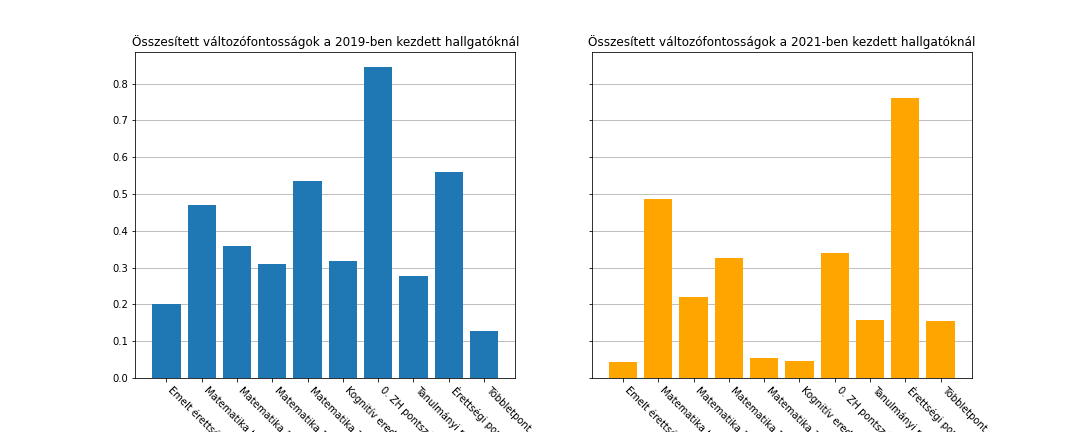
\includegraphics[scale=0.6]{kepek/eves_valtozok.png}
\caption{Az változók összesített fontossága a két évben}
\label{fig:variables2}
\end{figure}

\newpage

\begin{figure}[H]
\centering
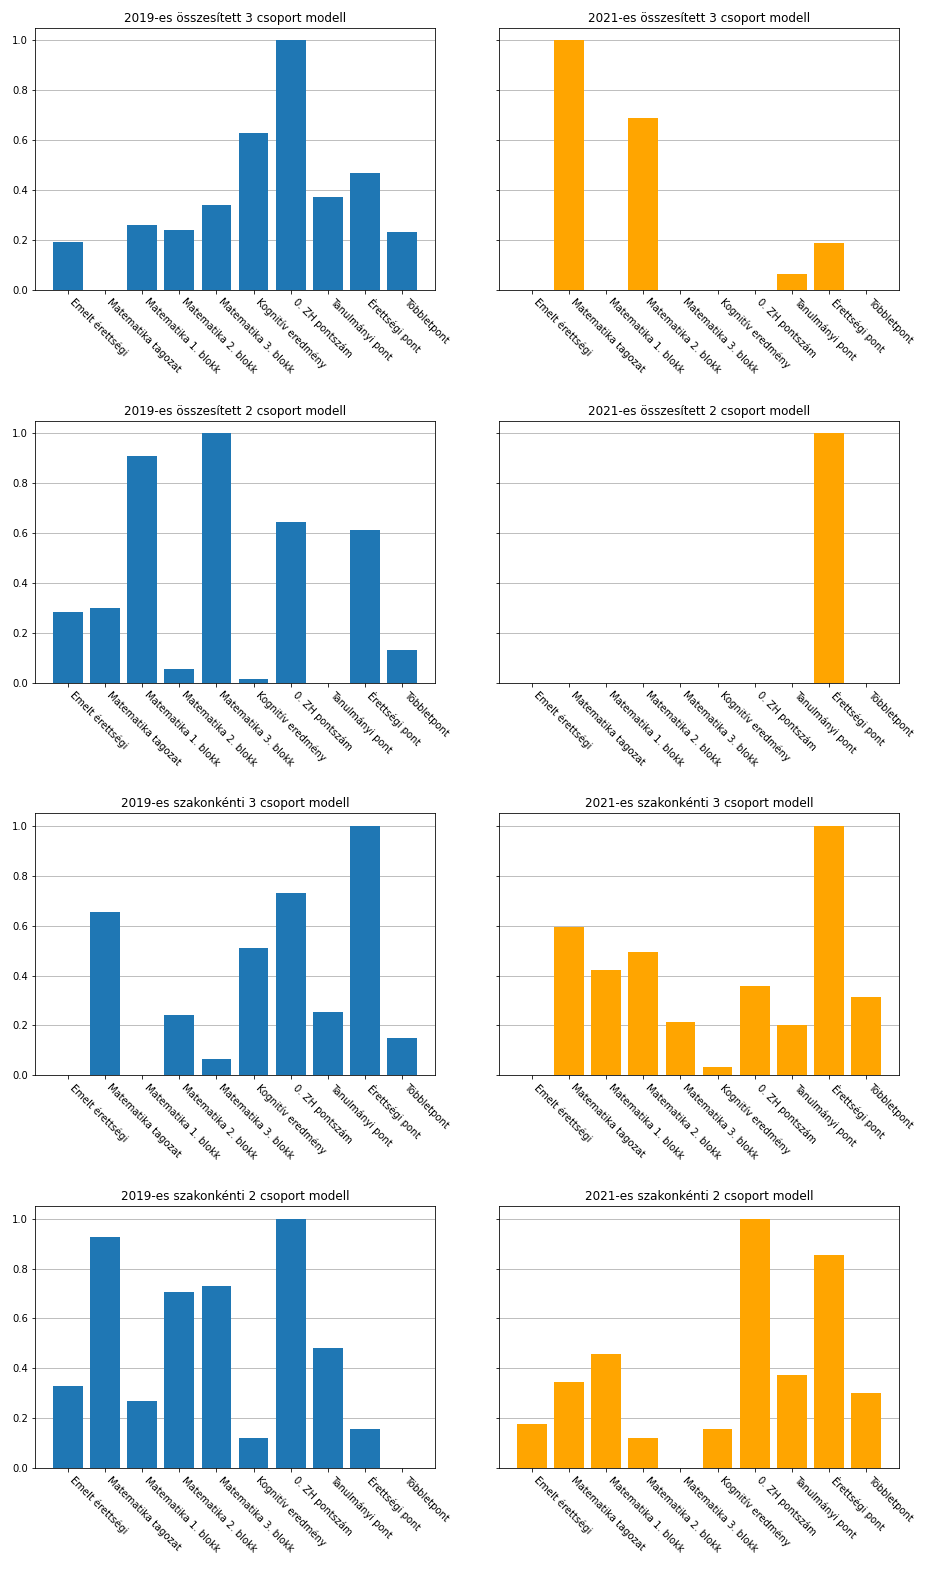
\includegraphics[scale=0.57]{kepek/modell_valtozo.png}
\caption{Az attribútumok prediktív ereje a legjobban teljesítő algoritmusoknál}
\label{fig:variables}
\end{figure}



%\newpage
%\begin{center}
%\begin{tikzpicture}
%	\draw (-10,-10) rectangle (-7,-9);
%	\draw[->] (-7,-9.5) -- (-5,-9.5);
%	
%\end{tikzpicture}
%\end{center}



A diagramokon szereplő értékek az egyes algoritmusoknál megállapított változófontosságok \textit{min-max} skálázott értékei, amelyeket regressziós algoritmusoknál az attribútumokhoz rendelt súlyokból, a többi osztályozónál pedig az Sklearn \textit{'inspection'} csomagjának segítségével nyertünk ki. Az összesített ábrán az egyes évek legfontosabb attribútumai a megfelelő évek különböző modelljein is többnyire jelentős szignifikanciával bírnak, a többi változó fontossága viszont modellenként eltérő. A 0.ZH pontszám illetve az érettségi pont prediktív ereje mindkét évben kiemelkedő. A 2019-es évben a matematika tagozaton való jelenlét és a kognitív teszten elért eredmény is nem elhanyagolható szignifikanciával bírt, viszont 2021-ben ezen tényezők prediktáló ereje csökkent, ugyanakkor az elért tanulmányi- és többletpontok jelentősége a matematika jegyre nézve több mint kétszeresére nőtt. Összevetve a felderítő adatelemzéssel, ezen eredmények arra engednek minket következtetni, hogy  ...

A kumulált átlag prediktálásának eredményei (statisztikák, reziduális szórásdiagramok és az egyes változók prediktív ereje egymáshoz viszonyítva) a \ref{fig:kumulalt}. ábrán láthatóak. 

\vspace{0.5cm}



\begin{figure}[H]
    \centering
    \begin{minipage}[b]{0.4\textwidth}
    \begin{center}
    \textbf{2019}
    \end{center}
    \raggedright
    - $R^2$: 0.5462 \\
    - $MAE$: 0.3455 \\
    - $RMSE$: 0.4165 \\
    	\centering
        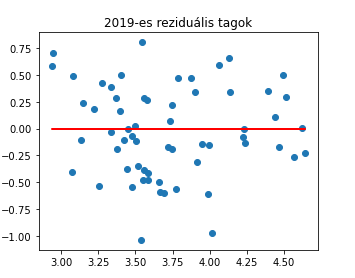
\includegraphics[width=1\textwidth, left]{kepek/residual2019.png} % first figure itself
        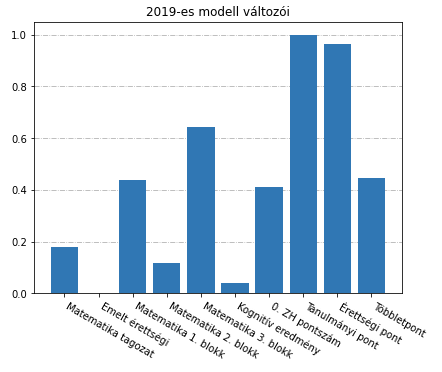
\includegraphics[width=1\textwidth, left]{kepek/kumulalt2019.png} % first figure itself
    \end{minipage}
    \begin{minipage}[b]{0.4\textwidth}
    \begin{center}
    \textbf{2021}
    \end{center}
    \raggedright
    - $R^2$: 0.5646 \\
    - $MAE$: 0.3710 \\
    - $RMSE$: 0.4415 \\
        \centering
        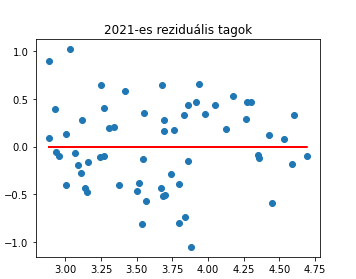
\includegraphics[width=1\textwidth, left]{kepek/residual2021.png} % first figure itself
        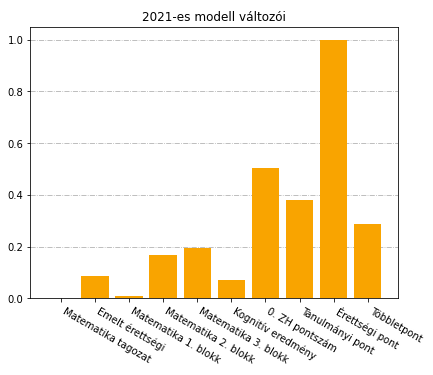
\includegraphics[width=1\textwidth, left]{kepek/kumulalt2021.png} % first figure itself
    \end{minipage}
   \caption{Lineáris regresszió eredménymutatói a két évben}
   \label{fig:kumulalt}
\end{figure}

Statisztikák tekintetében mindkét évben hasonló eredményeket kaptunk. Az értékekből arra lehet következtetni, hogy a modell

\begin{figure}[H]
    \centering
    \begin{minipage}[b]{0.4\textwidth}
    \begin{center}
    \textbf{2019}
    \end{center}
    \raggedright
    - $R^2$: 0.7485 \\
    - $MAE$: 0.3059 \\
    - $RMSE$: 0.4253 \\
    	\centering
        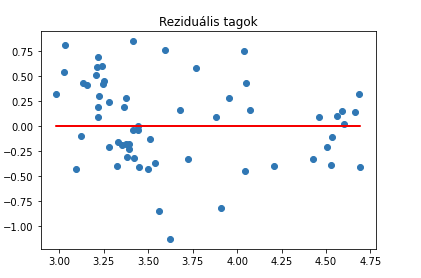
\includegraphics[width=1\textwidth, left]{kepek/residual2019_2.png} % first figure itself
        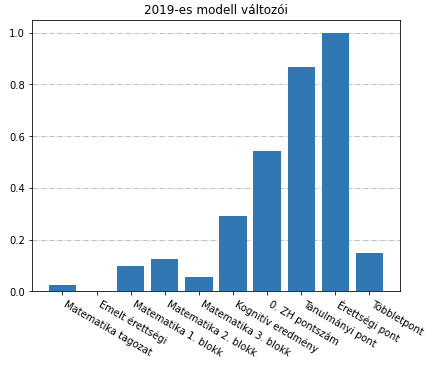
\includegraphics[width=1\textwidth, left]{kepek/kumulalt2019_2.png} % first figure itself
    \end{minipage}
    \begin{minipage}[b]{0.4\textwidth}
    \begin{center}
    \textbf{2021}
    \end{center}
    \raggedright
    - $R^2$: 0.4696 \\
    - $MAE$: 0.3770 \\
    - $RMSE$: 0.4407 \\
        \centering
        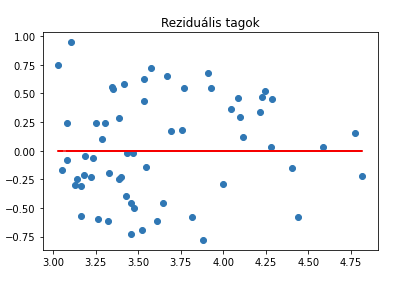
\includegraphics[width=1\textwidth, left]{kepek/residual2021_2.png} % first figure itself
        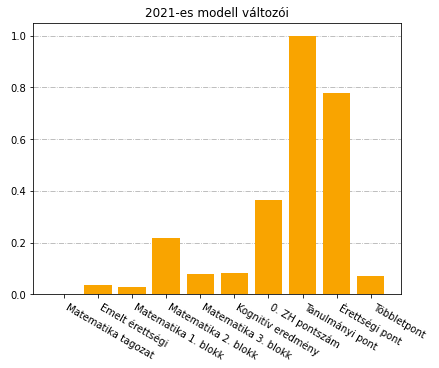
\includegraphics[width=1\textwidth, left]{kepek/kumulalt2021_2.png} % first figure itself
    \end{minipage}
   \caption{Gradient Tree Boosting eredménymutatói a két évben}
   \label{fig:kumulalt}
\end{figure}


\begin{thebibliography}{9}
\end{thebibliography}

\end{document}

